\documentclass{l4proj}
\usepackage[utf8]{inputenc}

\usepackage{listings}
\usepackage{color,soul}
\usepackage{xcolor}
\usepackage{enumitem}
\usepackage{graphicx}
\usepackage{subcaption}





\graphicspath{ {images/} }



\title{Go - Project}
\author{Jude Haris}
\date{May 2019}

\begin{document}
\maketitle

\pagenumbering{arabic}

\chapter{Introduction}
Go Life \& Death (GoLD) is a program developed in Java which can solve Go problems. The ancient game of Go is regarded as the oldest board game still being played in the modern day. The origins of Go are not completely known but it is said to be invented in China 3000-4000 years ago. The game has very simple rules and by most official rulesets played on a 19x19 board. Each player takes turns placing a black or white stone on the intersections of the grid lines on the board. There are 361 intersections on the Go board whereas Chess’s only has 64 squares to play on. The size of the Go board is a key factor in this project. Due to increased board size compared to most western board games, a computer will take significantly more time to search through each valid move in every turn of the game to determine the final outcome. On the other hand, the basic principles of the game are much simpler to program and execute in software. Some complicated rules such as self-capture and Ko rules do exist. While implementing these rules can be simple, the effect of them being implemented correctly is great. For instance, without implementing the Ko rule it would be impossible to make progress while searching Go’s game tree. Some situations occur where it becomes optimal for both players to repeat the same moves over and over in order to capture a single point on the board.  This would lead to a never-ending battle for the same point on the board without the existence of the Ko rule which forbids this to occur. Therefore without a correct implementation, any type of game tree search algorithm used to solve the board position would get stuck in these situations and loop infinitely. This project implements Go to allow the user to not fully play the game of Go but rather solve Go problems.
\section{Motivation}
The simplicity of the game's rules is deceiving, anyone can learn the rules of the game within 5-10 mins and will be able to play a full game of Go. The game's strategy and tactics are incredibly complex compared to the rules. Go players agrees with the sentiment that, to learn the game it takes little time but to become an expert or remotely good at it takes years maybe even decades. Due to the nature of the size of the board, the possible number of different games that could be played out in Go is inconceivably large. For a computer to calculate the perfect move via searching every valid move that could occur would take too long to be considered viable, not months or years but rather millenniums.

The current best AI built to play Go is AlphaGo [9] and its successors built by Google’s DeepMind team. It has defeated some of the world’s best Go players such as Lee Sedol during a challenge match in South Korea dropping only 1 game out the 5 played. AlphaGo has also defeated Ke Jie another highly ranked player in 2017 at Future of Go Summit winning all three games played. AlphaGo uses Monte Carlo Tree Search along with neural networks to evaluate different board positions and calculate the best move according to what it has learned through machine learning. With that in mind, AlphaGo is yet to be anywhere near perfectly solving Go due to the enormous complexity and possibility of moves, the team working on it is still finding ways to improve it.

The main motivation behind this project is to create a tool for Go players to enhance their skill at a certain aspect of Go. It is not to create an AI which plays whole games of Go but to create an AI which can play Life and Death problems and solve them.


\section{Aim}
The aim of this project was to create a tool program for Go players, from beginners to experienced which allows them to practise life and death problems and in doing improve their overall skill level at the game.  The aim also includes that the tool should contain an AI to play against its users in Go, which can identify all the valid moves and play the correct move given a board position.

Specifically, the project’s aim was to create a program which given a life and death problem for Go it would solve it. If the problem is solvable,  the AI should play the move which solves the problem otherwise it should play the move that it thinks is the best possible. The project was divided into two big milestones to keep track of the progress.

The first milestone within the project was to implement a substantial number of features, enough to let the users create problems and view them. This included implementing the rules of Go, having the ability to place stones and also to implement the bare bones of the AI which would be altered in the second part of the project to implement heuristics. This meant to implement a simple tree search which would be able to choose and play the correct move given infinite time or a problem small enough so that every valid sequence of moves could be searched. Other features such as loading and saving problem files were also part of the aim for the first milestone.

The second milestone was to alter and enhance the tree search implemented in the first milestone to be able to solve larger and complex problems. To achieve this GoLD needed a way to limit the search space hence decreasing the time taken to search but also creating uncertainty of choosing the best move. The aim for the second milestone was to introduce heuristics to determine how favourable a board position is after searching for certain depth into the possible sequence of moves and then picking move which leads to the most favourable board position. The overall goal of the second milestone was to enable GoLD to solve more realistic problems in a viable time frame for users to use the program without waiting too long.

\section{Project Outline}

Here is a short summary of each following chapters:

Chapter 2 Background \& Related Works – Explains key concepts which are used within the project, introduces Go and some relevant details of Go in more detail. Also looks at some similar work done.

Chapter 3 Requirements – Deals with expressing the functional requirements of GoLD and also some non-functional requirements.


Chapter 4 Design – Goes in depth about the AI and the tree search used with GoLD.  Explores the heuristics used to enable the GoLD to limit time spent searching the game tree. This includes board evaluation, move ordering and move generation.

Chapter 5 Implementation – Talks about the key features of GoLD and how they are implemented. Goes into some detail on how the Go board is represented within the program. Explains the pattern matching functionality used during board evaluation and move generation.

Chapter 6 Evaluation – Contains result of Beta testing and analyses of it. Also evaluates the performance of GoLD for every problem within the problems folder provided to beta testers. Goes into detail about the unit tests designed and tested to prove the correctness of the program.

Chapter 7 Conclusion – Concludes the whole paper by looking at the successes of the project, places of improvements and any possible future work.





\chapter{Background \& Related Works}
In order to achieve the aim of creating a tool program, a certain level of knowledge of the game of Go was required. Knowledge such as the rules of Go and details regarding life and death problems were important factors while designing and implementing GoLD. Along with understanding Go, researching papers and finding inspiration from similar work done was important for the progression of this project.
Go is a complex board game where the rules are far simpler than the strategies and tactics used to play it. To understand Go in general like how a beginner would,  was crucial in the progression of the project. To begin with, many simple questions needed to be answered about the game and how it is played in order to design GoLD. Basic concepts and terminology needed to be understood before tackling complex strategies which are built up from these basic concepts.

\section{Rules}

While there are no official rules for Go and many varied rulesets being used around the world, they are all quite similar. None of them really affect the strategy or tactics used within the game hence comprehending one ruleset was enough to understand the game in order to implement the rules within GoLD. This is especially true because the GoLD does not require counting scores which is the part of the rulesets that vary the most. The basic rules according to Japanese Rules of Go set by Nihon Kiin translated by James Davies [1] were used to define the basic ruleset used within the project. Some alterations were made to these rules to suit the problem-solving nature of the project rather than playing a whole game of Go which will be explained in a later section.

\begin{figure}[!ht]
\centering
\begin{subfigure}[b]{0.25\textwidth}
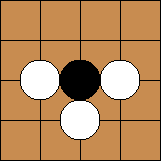
\includegraphics[width=\textwidth]{ex/Ex1-0.png}
\caption{Before Move}
\label{fig:ex1-0}
\end{subfigure} \qquad\qquad\qquad
\begin{subfigure}[b]{0.25\textwidth}
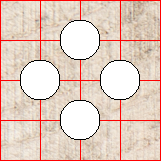
\includegraphics[width=\textwidth]{ex/Ex1-1.png}
\caption{After Move}
\label{fig:ex1-1}
\end{subfigure}
\caption{The black stone is “captured” when the white stone at the top is placed because the black stone loses its last liberty}
\label{fig:ex1}
\end{figure}

The basic rules of Go are as follows:
\begin{enumerate}

  \item Initial Go board is empty containing no stones unless handicaps are applied.
  \item Black plays first and then white. Players take turns alternately placing stones of their own colour.
  \item The board contains a 19x19 gridline pattern with 361 intersections. Stones are played on the intersections and not the square in between. Stones can only be played on empty intersections. These intersections are also referred to as points on the board.


  \begin{figure}[!ht]
  \centering
  \begin{subfigure}[t]{0.25\textwidth}
  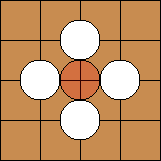
\includegraphics[width=\textwidth]{ex/Ex2-0.png}
  \caption{Middle point is invalid for black to play}
  \label{fig:ex2-0}
  \end{subfigure}  \qquad\qquad\qquad
  \begin{subfigure}[t]{0.375\textwidth}
  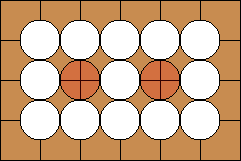
\includegraphics[width=\textwidth]{ex/Ex2-1.png}
  \caption{Both middle points are invalid for black to play}
  \label{fig:ex2-1}
  \end{subfigure}
  \caption{A black stone cannot be placed in the middle of both of these shapes because it would lead to self-capture.}
  \label{fig:ex2}
  \end{figure}

  \item Each turn consists of few parts as follows:
  	\begin{enumerate}[label={(\alph*)}]
		\item Current player is to place a stone of their colour on an empty intersection of their choice.
		\item Then all opponent’s stones that do not have a liberty is removed from the board. See ~\autoref{fig:ex1}.
		\item A move is invalid if it will cause one or more stone of the current player’s colour to be captured – this is to prevent self-capturing moves. See ~\autoref{fig:ex2}.
		\item Removal of the opponent’s stones takes precedence over the self-capture check. This allows for moves which capture opponent’s stones but is suicide if the opponent’s stones are not removed first. See ~\autoref{fig:ex3}.
	\end{enumerate}

    \begin{figure}[!ht]
    \centering
    \begin{subfigure}[b]{0.25\textwidth}
    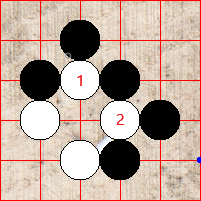
\includegraphics[width=\textwidth]{ex/Ex3-0.png}
    \caption{Before Move}
    \label{fig:ex3-0}
    \end{subfigure} \qquad\qquad\qquad
    \begin{subfigure}[b]{0.25\textwidth}
    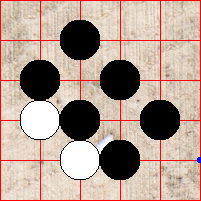
\includegraphics[width=\textwidth]{ex/Ex3-1.png}
    \caption{After Move}
    \label{fig:ex3-1}
    \end{subfigure}
    \caption{A black stone can be placed in the middle of the four white stones because 1 and 2 will be immediately captured before the self-capture rule is applied. }
    \label{fig:ex3}
    \end{figure}

    \begin{figure}[!ht]
    \centering
    \begin{subfigure}[bt]{0.25\textwidth}
    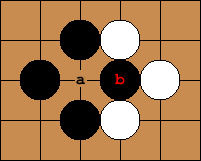
\includegraphics[width=\textwidth]{ex/Ex4-0.png}
    \caption{Before Move}
    \label{fig:ex4-0}
    \end{subfigure} \qquad\qquad\qquad
    \begin{subfigure}[bt]{0.25\textwidth}
    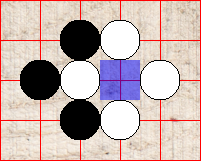
\includegraphics[width=\textwidth]{ex/Ex4-1.png}
    \caption{After - Blue Square is Ko}
    \label{fig:ex4-1}
    \end{subfigure}
    \caption{ Once a white stone is placed at a to capture the black stone at b, a black stone cannot be played at b next turn by the opponent to capture the white stone placed at a.}
    \label{fig:ex4}
    \end{figure}

  \item Ko rule – Player is not allowed to place a stone on point A if it will capture exactly one opponent stone which was placed on point B during the opponent’s previous turn. This rule only applies if the opponent in the previous turn captured exactly one stone on point A. This is to prevent an infinite repetition of the same few moves. See ~\autoref{fig:ex4}.

  \item The game is over when both players pass consecutively and the player with more territory wins. (Scoring can be complicated but is irrelevant to understand the basic rules)

\end{enumerate}




\section{Rules for GoLD}
The rules stated in the previous section outline all the important rules of Go. Some of these rules are slightly altered in order to suit the problem-solving environment set in GoLD.

The alterations are as follows:
\begin{enumerate}

\item The initial board is set up to represent a life and death problem - should be a valid initial board position.
\item Not all 361 intersections can be played on – boundaries are set by the creator of the problem
\item For the purpose of these problems, one player is considered to be the attacker and the other to be the defender.
\item Attacking player is not able to pass unless the attacking player has no valid moves and the Ko rule is restricting play.
\item Two consecutive passes do not end the game/problem.
\item The problem is solved when the attacking player has no valid moves and cannot pass, if the keystones are still on the board then the defending players have won. Otherwise, the problem is solved if all the keystones are captured hence the attacking player has won.

\end{enumerate}


\bigskip
A valid initial board state is defined by the following :
\begin{itemize}
\item Contains at least one keystone
\item All keystones are the same colour
\item Must have a valid empty intersection to play on within the boundaries set for the problem
\item Can only contain up to one point of Ko
\item Stones that have no liberties cannot exist on the board
\end{itemize}

\bigskip
In a normal game of Go, there are no boundaries set on the board, every intersection on the board is playable if the other rules allow it. To achieve the aim of this project there is a definite need for boundaries to be set on the board for each problem. Without doing so, the number of valid moves required to be searched by the AI would be too large to determine the best move in a limited time. To set boundaries during the creation of a problem, the creator can deem relevant points on the board as "valid points" to play on. Any points on the board with preplaced stones are also regarded as within the boundary. For example, a black stone is captured, the empty point remaining will be regarded within the boundary of play. It can be very difficult or even impossible for a problem creator to determine all relevant points for the problem. GoLD leaves it in the hands of the problem creators to define life and death problems with relevant boundaries. This is a crucial trade-off which is required to allow the program to be able to find the correct answer in a feasible time.
The reason behind the 4th alteration to the basic rules is to restrict infinite passing which would be allowed due to the 5th alteration. Attacking player is allowed to pass under the circumstance that they have no valid moves and an empty intersection is invalid to play on due to the Ko rule, this resolves some rare occurrences where boundaries set by the creator of the problem restricts the attacking player from winning.




\section{Go Terminology}

Throughout this dissertation many terms are used to describe various aspects of Go, some of which are commonly used term within the Go world and others are created for the purpose of this project.

Keystones – Set of predetermined stones which are used as the objective of the problems. These stones are to be captured by the attacking player and kept alive by the defending player.

Attacking player – In terms of life and death problems, the attacking player is the one which is trying to capture the keystones on the board.

In terms of life and death problems, the defending player is the one which is trying to keep the keystones alive on the board.

Board position – Refers to the entire state of the board, not just a single point on the board.

Valid points – Set of predetermined intersections that are allowed to be played on for the given the problem. A valid point can also refer to a point which the current player is able to play on.

Connected - Two stones are connected if they are of the same colour and is adjacent to each other or there is a set of stones of the same colour which is connected to both stones.

String – Set of stones of the same colour which are connected.

Keystring – Any string which contains one or more keystones.


Liberty - The liberties of a stone are all adjacent empty intersection of the stone and all adjacent empty intersection of any stone connected to the original stone. See ~\autoref{fig:ex5}.






\begin{figure}[!ht]
\centering
\begin{subfigure}[b]{0.25\textwidth}
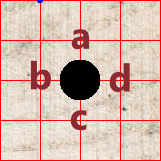
\includegraphics[width=\textwidth]{ex/Ex5-0.png}
\caption{One Stone's liberties}
\label{fig:ex5-0}
\end{subfigure}\qquad
\begin{subfigure}[b]{0.375\textwidth}
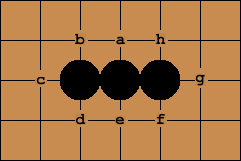
\includegraphics[width=\textwidth]{ex/Ex5-1.png}
\caption{Stone string's liberties}
\label{fig:ex5-1}
\end{subfigure}
\caption{The liberties of a stone or a string of stone are the empty adjacent intersections.  In ~\autoref{fig:ex5-0} intersections a,b,c and d are the liberties of the black stone.
In ~\autoref{fig:ex5-1} intersections a to g are the liberties of the black stone string but h is not a liberty due to the white stone that occupies it.}
\label{fig:ex5}
\end{figure}


Atari – String is in Atari when it only has one liberty.

Atari Point – The last remaining liberty of a string.

Ko Point –  An empty intersection which is restricted from play due to the Ko rule

Seki – Two strings of opposing colour that are alive next to each other. Neither player can capture the opponent string without first sacrificing their own string.





\section{Life and Death Problems}

Life and Death is an essential part of Go. Life and Death is the term used to describe the battle that takes place to either attack and capture enemy stone strings or to defend and keep alive ally stone strings. Situations on the board where it becomes crucial to defend one’s own stone strings or capture enemy ones arrive very often. During the end game in Go, the ability to win these battles with as much territory as possible will decide the victor. Beginners are highly recommended to understand and learn how to play out these battles as they are clear deciders in the game. Many of the literature on Go is purely based around providing life and death problems and explaining the importance of them and how to tackle such situations appropriately.[3][4] The purpose of GoLD is to create a tool which helps players to understand and solve these problems.

\subsection{Dead, Alive or Unsettled}

The three main ways to describe the status of a string are alive, dead or unsettled. To deduct accurately the state of a group of stone can be difficult and requires a lot of experience and knowledge about the possible moves that could be made and the counter plays to them and the result of counter plays.

\begin{figure}[!ht]
\centering
\begin{subfigure}[b]{0.45\textwidth}
\includegraphics[width=\textwidth]{LD/1a.png}
\caption{Before Moves}
\label{fig:LD-1a}
\end{subfigure}\qquad
\begin{subfigure}[b]{0.45\textwidth}
\includegraphics[width=\textwidth]{LD/1b.png}
\caption{After Moves}
\label{fig:LD-1b}
\end{subfigure}
\caption{Straight Four in the corner is alive}
\label{fig:LD-1}
\end{figure}

A group of stones are said to be alive if the group cannot be captured even if the opponent is to play first. To expand on this, even if opponent plays a move which threatens the group of stone there is always a responding move which will in turn keep the group of stones alive. ~\autoref{fig:LD-1} shows an example of white group which can be deemed to be alive, if black first plays at 1 then white will play at 2, if black first plays at 2 then white will play at 1 both outcomes will lead white group having two eyes.

\begin{figure}[!ht]
\centering
\begin{subfigure}[b]{0.3\textwidth}
\includegraphics[width=\textwidth]{LD/2a.png}
\caption{Before Moves}
\label{fig:LD-2a}
\end{subfigure}\qquad
\begin{subfigure}[b]{0.3\textwidth}
\includegraphics[width=\textwidth]{LD/2b.png}
\caption{After Moves}
\label{fig:LD-2b}
\end{subfigure}
\caption{Square Four in the corner is dead}
\label{fig:LD-2}
\end{figure}


A group of stones is said to be dead if the group can be captured even if the group’s colour can play first. A white group is deemed dead if white can play the first move and black has a responding move which will keep the white group in a dead state. ~\autoref{fig:LD-2} shows a group of dead white stones, for this group to live it requires white stones on two points diagonally opposite to each other and no white stones on the other two points. For example, if white can play at a and d then it becomes alive. This is impossible to achieve as black can respond to white’s initial move by playing at diagonally opposite point seen in~\autoref{fig:LD-2b}.


A group of stone is said to be unsettled when the group is alive if the group’s colour can play first but dead if the opponent plays first. Groups which are unsettled are crucial to the outcome of the board, whoever can play first near the group can determine who controls the whole territory the unsettled group surrounds. ~\autoref{fig:LD-3} shows an unsettled white group which has a vital point at a where if white plays first at a then the group achieves two eyes and is alive. On the other hand, if black plays first at a then white cannot achieve two eyes hence it becomes dead.

\begin{figure}[!ht]
\centering
\begin{subfigure}[b]{0.4\textwidth}
\includegraphics[width=\textwidth]{LD/3a.png}
\caption{Vital point at a}
\label{fig:LD-3a}
\end{subfigure}\qquad
\begin{subfigure}[b]{0.4\textwidth}
\includegraphics[width=\textwidth]{LD/3b.png}
\caption{White lives with 2 eyes}
\label{fig:LD-3b}
\end{subfigure}
\caption{Straight Three on the side is unsettled}
\label{fig:LD-3}
\end{figure}




\subsection{Eyes}
The concept of an eye is key in understanding life and death problems and Go in general. There are no perfectly defined statements on what an eye is but in general, an eye is a space surround by a group of the same colour. Single eye point shapes are shown in ~\autoref{fig:LD-4}. In these shapes, the stones surrounding the eyes are important if any of them are missing then the eye will no longer be a real eye. An important deduction about a single point real eye is the fact opponent cannot play on the single point eye unless the eye is only liberty of the surrounding stones. If two real eyes are connected by the same group of stones, then it becomes impossible to capture that group of stone unless the eyes are covered up by its own colour. These groups of stones are unconditionally alive which means even if the opponent is able to play multiple times in a row the group cannot be captured. ~\autoref{fig:LD-3b} shows an example of a group of white stone which contains two eyes at a and b, due to the self-capture rule black can never place in a without having a stone at b and same applies of b hence the white group in unconditionally alive.

\begin{figure}[!ht]
\centering
\begin{subfigure}[b]{0.3\textwidth}
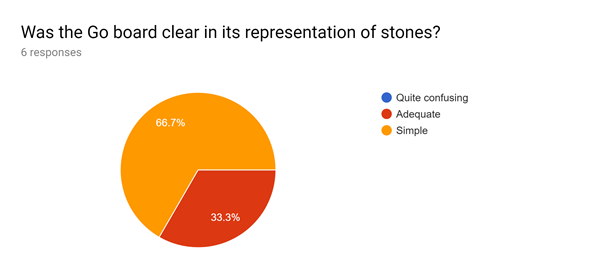
\includegraphics[width=\textwidth]{LD/4.png}
\caption{Different Single Point Eyes}
\label{fig:LD-4a}
\end{subfigure}
\caption{Single Point Eye in the middle, side and corner}
\label{fig:LD-4}
\end{figure}



In cases of larger groups which surround more empty points, these empty points are referred to as the eye space. The eye space of a group is important in determining early on within a game whether a group is dead or alive. An eye space can be reduced to create real eyes, the greater the amount of eye space a group surrounds the greater the ability it has to create two real eyes and live unconditionally.

When eyes are not fully developed on the board for example at a in ~\autoref{fig:LD-5a} they are deemed to be half eyes, depending on who plays first at b decides whether a real eye is formed or is stopped from being formed. Half eyes are important because two half eyes add up to one eye.  A group such as the one shown in ~\autoref{fig:LD-5b} which has a real eye at a and two half eyes at b and c can be deemed as alive due to the fact that when black plays 1 to deform one half eye white can play 2 to fully form the other half eye into a real eye creating an unconditionally alive group.
\begin{figure}[!ht]
\centering
\begin{subfigure}[b]{0.4\textwidth}
\includegraphics[width=\textwidth]{LD/5a.png}
\caption{Vital point at a}
\label{fig:LD-5a}
\end{subfigure}\qquad
\begin{subfigure}[b]{0.5\textwidth}
\includegraphics[width=\textwidth]{LD/5b.png}
\caption{White lives with 2 eyes}
\label{fig:LD-5b}
\end{subfigure}
\caption{Straight Three on the side is unsettled}
\label{fig:LD-5}
\end{figure}


\subsection{Outcomes of Life and Death}
The possible outcomes of some life and death situations are not as obvious it would seem. There are different types of life and death results. The solution found for a problem can vary the result of the whole board depending on which the following categories it fits into.
Unconditional life or escape into the centre of the board is the best outcome a defending player can expect, this means their group of stone will be scoring them the points without uncertainty. Another but a lesser type of victory is life through Seki, which means mutual life, this is where two groups opposing colour of stones live sharing liberties and neither player can try to capture the opponent’s group because it will lead to their group’s death first. When an attacking group of stones is able to live in mutual life along with the defending player’s group then the outcome is slightly less favoured than unconditional life due to the end game scoring. In isolated life and death problems and for the purpose of GoLD this difference between unconditional life and Seki is not taken to account, Seki is deemed victory for the defending team.

Life and death problems can also conclude where Ko occurs within the area, in the full game of Go this is very important in deciding Ko fights in other parts of the board and can be seen as leverage to be used.  For the purpose of GoLD and in isolated problems these situations are further played on until a defining end is met where the group is dead or alive. The final possible result is death where the defending player’s group is captured without any Ko situation which the best-case scenario for the attacking player.


\section{Related Works}

Martin Müller's Explorer [2] was a strong program developed with the intention of playing Go. In his paper, he delves into some key aspects of Explorer which have been useful to comprehend some ideas behind creating a Go-playing software. He describes the importance of board evaluation within a tree search algorithm such as minimax.

Explorer can evaluate certain areas of the board in terms of safe territories for each player and can distinguish between safe stones and safe territories. Safe stones are any stones that are deemed alive but safe territories requires that opponent stones cannot live within the safe stones. Explorer also takes into consideration of Semeai positions which are capturing races that occur within Go. The victor of Semeai can be determined early sometimes and hence doing so during the evaluation could save searching further during a tree search algorithm. Müller also goes into detail about his zone-based evaluation where Explorer is able to distinguish areas which are in conflict and areas which are clearly controlled by a certain colour.

While Explorer aims to play Go, this project aims to create a program to solve life and death situations. To do so, determining the safety of keystrings within a problem is important. Explorer's methods of recognising safe strings such as Benson's algorithm [10] and also the improved version of the algorithm described in [11] were regarded during the initial design of GoLD.

Work done by Ken Chen and Zhinxing Chen [11] in creating Go Intellect and HandTalk were also quite interesting and relevant while working on this project. The key aspects of their work regarding eyes and determining the value of a shape of stones depending on the number of eyes the shape can produce was great a motivator during the implementation of GoLD's pattern-based heuristics.
Another relevant work researched during this project was Adrian B. Danieli's paper [12] on his own TsumeGo problem solver. In his paper, he explores in-depth the process in which his program was developed. Explanation of key concepts such as move generation and board evaluation were helpful in understanding how to develop my own work. A particularly relevant piece of information which was used as advice during the design of GoLD was that there was a problem in his representation of each node during the tree search. He believed his representation of each node caused extra workload during tree search without a good reason to do so. He goes on to explain due to the depth-first nature of his program "compressing" and "decompressing" the board positions for every node was waste of time. Rather than saving some space which is not as relevant when using a depth-first search, it would have been better to save time by storing the entire board position for each node.








\chapter{Requirements}

The project needed a well-defined list of requirements to outline key features and help with the implementation order of those key features. Time constraints and the resources available had to be taken to consideration before further work on the project was done. From the start, the project was divided into two major milestones each containing a set of requirements to achieve the milestone. These milestones were set up to help evaluate the progress throughout the project and also to help streamline the workflow throughout the project so that at all points there was a goal to strive towards. The functional requirements identified earlier on the project captured most of the work required but throughout the project, these requirements were refined and added to in order to solve unseen problems that arose during the project duration. Some non-functional requirements were also discovered earlier on which were used to refine the goals of the project.

\section{Functional Requirements}

\subsection{Milestone 1}
The project's first milestone's aim was to implement most of the key features required for users to create and view problems. In addition to this, the aim consisted of enabling the computer to play moves according to a simple tree search. This milestone consisted of the following requirements.

\subsubsection{Go Board}
The first milestone required a Go board which the user and the computer will be able to interact with. This meant there was a need to implement a Board object which is capable of storing relevant data and contained methods which are able to process the relevant data.

The relevant data needed to include the following:
\begin{itemize}
\item A representation of all the points on the board
\item Current turn
\item All of the stone strings for both colours
\item Colour of keystone
\item Point of Ko
\item Lists of Atari points for both colours
\item List of valid moves for the current turn
\end{itemize}

The relevant methods which are able to do the following were required:
\begin{itemize}
\item Make a move on the board and update the entire board accordingly
\item Generate all the valid moves for the current turn
\item Check if a move is valid – this should include self-capture check and Ko check
\item Check for capture and remove stones accordingly
\item Obtain all the liberties of a given stone string
\end{itemize}

\subsubsection{Play Mode}
Play mode is the screen in which the user can load a problem up and play through it. Play mode needed to contain a Go board in order to display problems. The board itself needs to be interactable, the user should be able to click on valid points on the board to make a move.

Play mode also needed to contain buttons which do the following:
\begin{itemize}
\item Load a problem
\item Save a problem
\item Switch to editor mode
\item Tell the computer to start search for the best move of the current board position
\item Tell the computer to stop search
\item Reset the problem to how it was loaded
\item Undo \& Redo moves
\item Switch Turns
\item Pass the turn
\end{itemize}

\subsubsection{Editor Mode}
Editor mode is the screen in which the user can create problems from scratch or edit problems that are loaded in and then save them for future use. Similar to play mode, editor mode needs to contain a Go board in order to display the problem which is being created/edited. The board itself needs to be interactable, the user should be able to place stones by simply clicking on the points on the board. Editor mode also needed a way for the user to decide which stone is currently being placed or whether if stones are being removed when the user clicks on the board.
Editor mode also needed buttons to do the following functions:
\begin{itemize}
\item Load a problem
\item Save a problem
\item Switch to play mode
\item Set who plays first during the problem
\item To reset the board into an empty state
\item Rotate and flip the board
\item To place a keystone
\item Switch keystone colour
\end{itemize}

\subsubsection{Computer}
To achieve the first milestone the computer was required to perform a tree search. The tree search chosen for this project was the Alpha-Beta pruning algorithm. The requirement for the computer was that it needed to produce the best move possible given infinite time and or small enough problem via searching every valid sequence of moves then interact with the board in play mode by making the best move found.

\subsection{Milestone 2}
The second milestone’s aim was to enhance the computer AI by introducing heuristics to allow the user to restrict the time the computer is able to search for the best move. To do this following the requirements were added on top of the requirements for the first milestone.

Play mode required an improved interface containing additional buttons to configure the parameter of the Alpha-Beta search used by the computer. Within the play mode, the user needed to able to toggle on and off depth limiting and breadth limiting. Play mode should also allow the user to increase or decrease the depth limit and the breadth of the search as they desire.
The computer’s requirement was that it should be able to limit the depth of the search according to the user’s choice. To do this it was required to introduce a board evaluation function. In order to allow the computer to limit the breadth of the search, it was required to introduce a move generator function which was able to generate a limited number of moves depending on the user’s breadth choice.

\section{Non-Functional Requirements}
Throughout the project, some non-functional requirements were discovered and needed to be addressed, the following categories were made to specify the different criteria GoLD need to achieve.

Performance / Time - Important concern was the time a user wants to spend during the process of solving problems using GoLD. Hence the time it took for the computer to make a move.

Usability - Another concern was the ease of use , whether the program is simple and understandable for untrained users.

Reliability – The program should be able to cope with any kind of user inputs and should maintain running without any failures or crashes

In order to test all three categories of these non-functional requirements the project also had an additional requirement of producing a folder of problems which can be used during the evaluation phase. This folder of problems was required so that beta testers could have a set of pre-defined problems to test the program on. The folder was also required in order to perform quantitate evaluation of GoLD during the evaluation process, to judge the level of difficult the program can solve and what length of time it takes to do so.





\chapter{Design}


\section{Tree Search}
GoLD allows the user to play against the computer which is one of the main requirements of the project. To create a computer which is able to play against a human, GoLD must be able to determine the best move out of all the valid moves in the given board position for the current turn. The simplest way to achieve this is by searching through the game tree and determining the end result of each valid move sequence of moves. The game tree consists of every single board position that is possible to occur from the current board position. Board position refers to the state of the entire board, where each stone is on the board , whose turn it is and also if there is an intersection of the board where the Ko rule is applied. Each subtree of the game tree is the result of making a valid move in the current board position. To determine the best move, every sub tree of the current board position needs to be explored until the resulting board position is a game ending state. This type of search where every sequence of moves is processed is referred to as a brute force search. The ability to “brute force search” Go’s game tree is essential to have in GoLD as it is the foundation to which rest of the program’s AI is built upon.

\subsection{Minimax}
The basis of finding the correct move within GoLD is the Alpha-Beta pruning search algorithm which is based on the Minimax search algorithm. In order to understand Alpha-Beta, it is essential to understand Minimax. Minimax is based on the idea of taking turns, and fundamentally how one player is trying to maximise their own score and the other player is trying to minimise the opponent's score by increasing their own. Minimax is perfect for searching Go’s game tree where two players are playing, and one player’s gains are directly linked to the other player’s losses. A simple implementation of minimax with no depth limit will search each valid move of the initial board position until a gaming-ending state occurs. Minimax will choose a move which results in victory even if the opponent plays perfectly if there is such a move. In terms of Go, if it is currently black’s turn then minimax will start the search as black and during the search will alternate between playing as black and playing as white until a game-ending state is reached. Each subtree of the initial game tree is searched until either a subtree (move) is found where white cannot avoid defeat or all the subtrees are searched.
\begin{figure}[!ht]
\centering
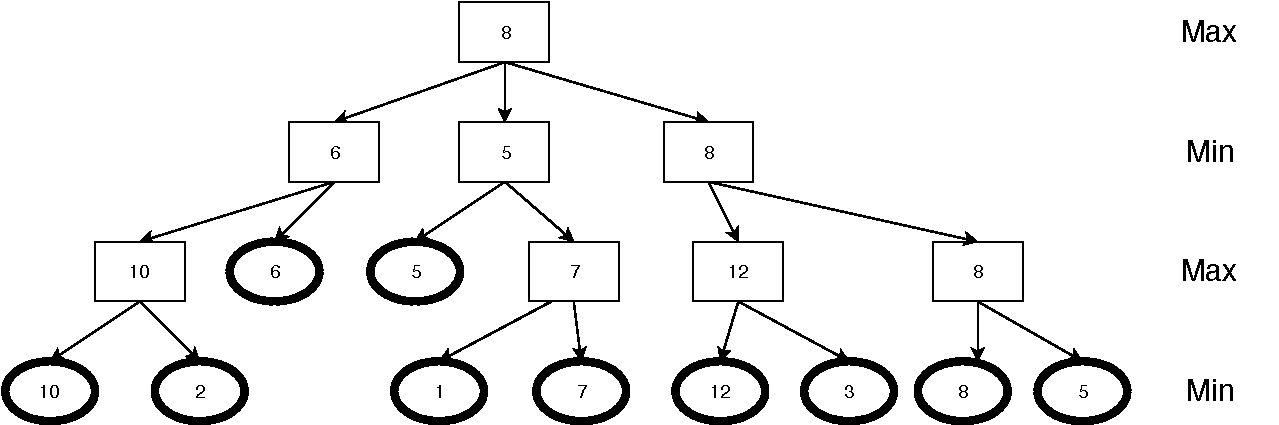
\includegraphics[width=0.9\textwidth]{MinMaxNumTree}
\caption{Minimax used for simple number game. Best score the maximizing player can get is 8. Even though scoring 10 and 12 are possible if the minimizing player plays optimally these scores cannot out be achieved.}
\label{fig:MinMaxNumTree}
\end{figure}

GoLD is only concerned with life and death situation in Go and hence it is simple to determine if the current board position is in a game-ending state. If the attacking player has no valid moves and the keystones, marked by the problem creator, remains on the board then the defending player has won. Alternatively, as soon as all the keystones on the board are captured then the attacking player has won. In a real game of Go, results of life and death situations are not so simple. There might be multiple solutions which result in the capture of all the keystones but there might only be one solution which will do so without allowing losses on other parts of the board for the attacking player. This is ignored within GoLD as we are only interested in the result of a life and death problem, and not the outcome of the board. Hence any solution which captures all the keystones are sufficient for the GoLD. ~\autoref{fig:MinMaxNumTree} show an example of minimax for a simple game where the max player tries to obtain the highest value and the min player tries to obtain the lowest value. Note the game-ending states are shown by a circular shape.

\subsection{Alpha-Beta Pruning Search}
The Alpha-Beta pruning algorithm is a smart improvement on the Minimax algorithm in order to reduce the search time. It allows for the same result to be determined without having to search through as many subtrees as Minimax does. It uses alpha and beta values to determine whether searching a subtree further ahead is a waste of effort or not. The search begins with the alpha value set to -inf and the beta value set to +inf. These values are passed down from the parent tree to each of its subtrees during the search. If a maximizing subtree finds a move which results in a score greater than the previous best score for that board position, then the alpha value of that subtree is increased to the value of the new best score. If a minimizing subtree finds a move which results in a score less than the previous best score for that board position, then the beta value of that subtree is decreased to the value of the new best score. After searching each move within a subtree, the algorithm checks if the alpha value is greater than or equal to the beta value and if it is then the algorithm decides that searching more moves within that subtree is pointless and returns the best score found so far back to the parent tree. These “beta cut-offs” reduces the search space for the algorithm by cutting off all the other moves from being searched. This amounts to a great improvement in search time compared to the minimax algorithm without changing the result. This is because the move that caused the beta-cut off to occur is worse than the parent tree’s best move found so far.

\begin{figure}[!ht]
\centering
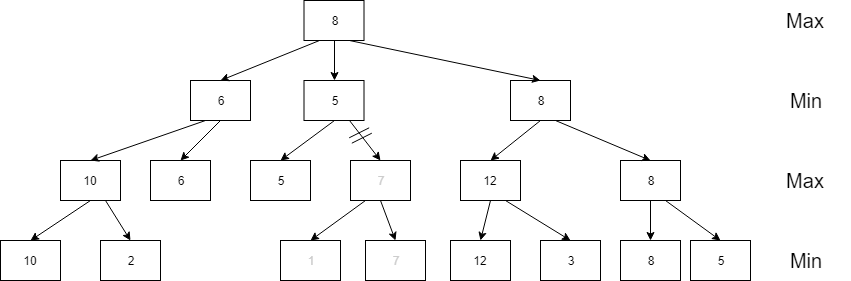
\includegraphics[width=0.9\textwidth]{ABNumTree}

\caption{The same simple number game as ~\autoref{fig:MinMaxNumTree} but using Alpha-Beta pruning. In the second subtree after searching the first move which returns 5, the algorithm cuts off from any further search in that subtree as it realises the first subtree will always be better than 5. }
\label{fig:ABNumTree}
\end{figure}


The following pseudocode addresses the Alpha-Beta pruning search algorithm with Go's Life and Death problems in mind. It was used for the initial design of GoLD's move finder function and later adapted to implement heuristics described in the following sections of this chapter.

\begin{algorithm}[H]
\caption{Alpha Beta Pruning Search}\label{Alpha-Beta}
    \DontPrintSemicolon
    \SetKwFunction{FalphaBeta}{alphaBeta}
    \SetKwProg{Pn}{Procedure}{:}{}
    \Pn{\FalphaBeta{$board,isDefending,depth,alpha,beta$}}{
         $depth\gets (depth+1)$\;
         $validMoves\gets (board.validMoves)$\;
        \uIf{keyStones.size = 0}{$\KwRet -\infty\;$}
        \uIf{(board.turn = attacking \textbf{and} validMoves.size = 0)}{$\KwRet { }\infty\;$}

        \eIf {isDefending}{
            $best\gets -\infty$\;
            \ForEach{move in validMoves}{
                board.makeMove(move)\;
                $score \gets alphaBeta(board,!isDefending,depth,alpha,beta)$\;
                board.undoMove()\;
                \lIf {($depth = 1$  \textbf{and}  $\mbox{score}<\mbox{best}$)}{$bestMove \gets move$}
                $best \gets max(best,score)$\;
                $alpha \gets max(alpha,score)$\;
                \lIf {$beta \leq alpha$}{$break$}
            }
            {$\KwRet { }best\;$}
        }{
            $best\gets \infty$\;
            \ForEach{move in validMoves}{
                board.makeMove(move)\;
                $score \gets alphaBeta(board,!isDefending,depth,alpha,beta)$\;
                board.undoMove()\;
                \lIf {($depth = 1$  \textbf{and}  $\mbox{score}>\mbox{best}$)}{$bestMove \gets move$}
                $best \gets min(best,score)$\;
                $alpha \gets min(alpha,score)$\;
                \lIf {$beta \leq alpha$}{$break$}
            }
            {$\KwRet { }best\;$}
        }
    }
\end{algorithm}





\section{Heuristics}

The Alpha-Beta pruning search algorithm by itself is a great improvement over the standard Minimax algorithm but even with this improvement, the sheer size of search space for a game tree can become quickly overwhelming for the search to handle in a reasonable time. Alpha-Beta even at best case has a complexity of $O(\sqrt{b^d})$ and at worst, $O(b^d)$  which means for problems with a higher number of initial valid moves or problems that require to search further ahead to come to a game-ending state could take an endless amount of time to search. For this reason, we have to introduce heuristics to allow the search to come to a quicker solution which could be incorrect rather than taking a long time to find a guaranteed correct solution. There are quite a few methods of implementing heuristics within the Alpha-Beta search, GoLD will be able to use few of these in combination or by themselves to restrict the time taken for the computer to respond to the user.

\subsection{Depth Limited Search with Board Evaluation}
A non-depth limited Alpha-Beta search will search deeper and deeper until a terminal state is found, this is very impractical for larger problems. Note that “depth” and “deeper” refers to how many moves ahead computer searches, the higher the depth the further ahead the computer has searched. Best way to deal with this is to introduce a depth limit where once depth X is reached the search is not continued. Of course, the problem with this is that when these depth cut-offs occur the board position will not be in a game-ending state and hence the Alpha-Beta search needs to do some type of evaluation in order to return a score which is between the two-opposing game-ending state of being dead or alive. The Alpha-Beta search will have to evaluate the board position when the cut-off depth is reached and return a value which represents how good the board is for the players. For example, if the board position will lead the attacking player to capture all the keystones then the board evaluation should return -5000,   on the other hand if the board position is in favour of the defending team then it should return 5000. Creating a function which evaluates the board accurately is a difficult task and doing so which can perform at the level of humans is even more difficult. An important factor to consider when designing an evaluation function is the time it takes to evaluate a board position. More complex the evaluation function becomes the longer it takes to evaluate single a board position hence the more time it takes to evaluate the board position every time the depth limit is reached.

\subsubsection{Pattern Matching Evaluation}

When evaluating a board position GoLD looks at the board similar to how humans would look at a board. It tries to identify general patterns on the board to give values depending on the pattern it finds. These patterns are based on the idea of eyes and eyes space. Identifying patterns which will lead to multiple eyes will be evaluated to give a very high score and hence the search will be able to recognise a group of stones which will be able to live without further searching. The general principle behind the patterns used in GoLD is to identify the number of eyes the pattern can yield when fully played out and values the pattern according to this factor. The values for each pattern found is added to the overall board score.

\begin{figure}[!ht]
\centering
\begin{subfigure}[b]{0.45\textwidth}
\centering
\includegraphics[width=\textwidth]{heur/1a.png}
\caption{Before}
\label{fig:heur-1a}
\end{subfigure}
\begin{subfigure}[b]{0.45\textwidth}
\centering
\includegraphics[width=\textwidth]{heur/1b.png}
\caption{After}
\label{fig:heur-1b}
\end{subfigure}
\caption{Straight Three in the middle of the board with missing corners.}
\label{fig:heur-1}
\end{figure}


Most of the patterns used within GoLD have a distinct feature which is common in life and death problems which is that depending on who plays first the pattern/shape becomes dead or alive. In other words, these shapes are unsettled and hence contains a vital point which will determine the number of eyes that can be produced by the shape. ~\autoref{fig:heur-1a} shows a pattern used in GoLD, the shape referred to as Straight Three but with its corner stones missing. The vital point of this pattern is a, if white is able to play at a then the pattern is almost ensured to create two eyes unless white makes a mistake filling in the corners. The corners b, c, d and e are also important for this pattern if black is able to have stones in both b and c  or in d and e then the wall of shape becomes weak and hence the shape can become captured. Due to alternating play if white plays first in this situation then it will be played out as shown in ~\autoref{fig:heur-1b} where white is able to produce two real eyes.


% Figure2
% The same pattern as Fig1 but on the side has similar properties but the safety of the shape requires white to have stones in both corners and the vital middle point.


\begin{figure}[!ht]
\centering
\begin{subfigure}[b]{0.45\textwidth}
\centering
\includegraphics[width=\textwidth]{heur/2a.png}
\caption{Before}
\label{fig:heur-2a}
\end{subfigure}
\begin{subfigure}[b]{0.45\textwidth}
\centering
\includegraphics[width=\textwidth]{heur/2b.png}
\caption{After}
\label{fig:heur-2b}
\end{subfigure}
\caption{Bent Three in the corner with a Single Point eye nearby  to connect.}
\label{fig:heur-2}
\end{figure}


An important insight into creating a better evaluation function is to recognise that patterns like the one mentioned above will be able to create a single point eye at the worst-case scenario. If the opponent is able to play at a pattern's vital point and restrict it from creating 2 eyes, the pattern will still be able to create 1 real eye which should be valued quite highly. By connecting two groups each containing a 1 real eye the defending player can achieve a live shape. When searched patterns fail to meet 2 eyes, GoLD stores the eye space of each failed pattern in a collection of eye spaces. This is because each of these eye spaces is highly probable to contain one real eye. Once the whole board is searched for all the different patterns used within GoLD and each identified pattern's values totalled, the evaluating function is left with the collection of eye spaces which all contain one real eye. Using this collection of eye spaces GoLD is able to group together multiple eye spaces which are connected through stones of the same colour. Any group of eye spaces that contains two or more unique eye spaces are identified as highly valuable due to fact that they will most likely produce two real eyes.

~\autoref{fig:heur-2} shows an example of where GoLD is able to recognise a new shape with 2 real eyes. Bent Three in the corner is about to lose its vital point once black plays at a but white can connect to the Single Point Eye nearby by playing at b. This creates a new shape which contains 2 real eyes. GoLD recognises that the Bent Three in the corner will create one real eye even though it has lost its vital point. When white connects at b, GoLD's eye space grouping algorithm identifies that the new shape contains at least 2 real eyes and hence will score the shape highly.

\begin{figure}[!ht]
\centering
\begin{subfigure}[b]{0.34\textwidth}
\centering
\includegraphics[width=\textwidth]{heur/3a.png}
\caption{Black Hanes at 1}
\label{fig:heur-3a}
\end{subfigure}
\begin{subfigure}[b]{0.45\textwidth}
\centering
\includegraphics[width=\textwidth]{heur/3b.png}
\caption{Black Cuts at 1}
\label{fig:heur-3b}
\end{subfigure}
\caption{Important type of moves}
\label{fig:heur-3}
\end{figure}



To limit time spent on board evaluation only a small number of unique patterns can be searched. Due to this constraint, it was important to identify the essential shapes/patterns which have the ability to create eyes. Fifteen different patterns ranging from a Single Point Eye to a Rabbity Six along with all their variations on the edges and corners of the board are used within GoLD.  Along with these patterns, the evaluating function also tries to identify stones which are placed in good positions with respect to the opponent stones. The evaluating function looks for areas of the board that are the result of a cut, hane or even simply connecting two groups of stones and awards values accordingly.



~\autoref{fig:heur-3a} shows a hane which is a move where a stone is placed next to an opponent stone which is already in contact with one’s own stone. Hane is a move which plays around one or more opponent stones. Note: playing at the opposite side of white here is not a hane.~\autoref{fig:heur-3b} shows a cut where black is able to stop white from connecting the two white stones by playing at 1.






\subsection{Move Ordering}
The benefit of Alpha-Beta pruning search over simple Minimax search is that when cut-offs occur a great number of subtrees of possible board positions do not need to be searched. Erik van der Werf talks about the importance of move ordering during Alpha-Beta search and the effects of good move ordering heuristics [5]. If the best move is always selected to be searched first, then the algorithm will produce cut-offs when all the other moves are searched afterwards. The idea behind this is if the best move is found first then all other moves will never return a score which is better than the best move. With this in mind, we can see that ordering the moves list to consider the best move first or even a move which will produce more cut-offs first, is a great way to reduce the number of board positions to search without altering the result.
\subsubsection{Killer Move Heuristic}
GoLD uses a deeply researched [6] method, Killer Heuristic, introduced by Huberman, B.J. [7] to order moves when searching through endgames of Chess using AB. Huberman’s theory was that a move (killer move) which led to a better board position from initial board position A will also lead to a better position from a similar initial board position B if the move is a valid move for B.  Using this theory, these killer moves should be searched first when a similar board position occurs during AB search. The moves which are considered killer moves are defined easily by using the cut-off characteristics of AB search, during the search if a move causes a beta cut-off to occur then this move can be considered a killer move and hence will be stored to be used for move ordering.  We can define a similar board position simply by looking at the depth in which the board position occurs in. Hence an ideal way to implement the killer heuristic is to store a number of moves for each depth which caused beta cut-offs to occur. Storing a great number of moves for each depth can lead to increased work during the move ordering process hence it is most effective only to store a few moves. GoLD only stores two killer moves k1 and k2  for each depth.

Move Ordering for a board position A which occurs at depth d consists of searching the list of valid moves for k2 of depth d and if k2 is a valid move in this board position then k2 is ordered to the top of the valid moves list. After which, the same is done for k1 of this depth(k1 is searched second in order to give k1 priority over k2). When a cut-off occurs at depth d then the k1 of that depth becomes k2 and the move that caused the cut-off to occur becomes the new k1 of depth d.

\subsection{Alpha-Beta with Iterative Deepening}
An issue with AB search is that if the best move is found at depth d then searching past depth d for the other branches is always a waste of time. For example,  black is to play and kill white. Moves A to E are the valid moves of the current board position and the moves will be searched in alphabetical order. If D is the best move and will result in a victory for Black at depth 3 then searching past depth 3 for move A, B and C is a waste of time. Without searching D first there is no way to obtain this information hence A, B and C will be searched to deeper depths. Iterative deepening is an effective method to work around this problem. Alpha-Beta with Iterative Deepening is a process in which AB search is performed multiple times and at each iteration, the depth limit is increased by 1. This cycle takes place until max depth limit is reached, or a favourable game-ending state is found  (in the example it would be white dead). This effectively alters AB search to only increment depth by 1 at a time and hence solving the problem of searching moves to deeper levels than not required.
The drawback of this process is that it requires multiple iterations of AB search and will have to perform redundant computation for the lower depths of the game tree. Work done by Korf R. [8] shows that redundant computation does not affect the overall time of the tree search as much as it would seem. In fact, using the result of each iteration to perform the next iteration can reduce the time taken to perform the next iteration and possibly the overall run time of the search. Each iteration will return the principal variation(PV) which is the sequence of moves which is considered to be the best determined by the search. The PV of the previous iteration will be set as the first sequence of moves the next iteration searches. This is another form of move ordering which effectively improves overall performance compared to a normal fixed depth limit search.
Due to the depth-first nature of the depth limited AB search, the search will not provide a result until every move is searched to a game-ending state or to the limited depth. This means the search will not be able to produce the best move searched so for if it is stopped in the middle of searching. Without the introduction of Iterative Deepening in GoLD’s search the user is not able to search for a limited amount of time, rather the user would have to predict which depth limit to set in order for the search to complete in the time they desire.  Predicting the depth limit could lead the user to set the depth limit too high which would lead the search to last longer than what the user would like. Iterative deepening fixes this issue by allowing the user to stop the search whenever they desire and to use the result of the last fully performed iteration to make the best move found so far hence improving the usability of the GoLD.


\subsection{Move Generator}
GoLD allows the creator of the problem to set the valid points of play on the board and any points on the board which contains a stone when captured become a valid point of play within the problem. A high number of valid moves to begin the problem with creates extremely large game trees which would take too long to search even with the best heuristic move ordering. The number of valid moves can be regarded as the breadth of the game tree. In order to limit the breadth of the game tree GoLD introduces a move generator.
The goal of a move generator is to pick out x number of moves from all the valid moves of the current board position in order to cut down the number of moves to be searched. A perfect move generator will always pick the best move if it could only pick one move to generate but this is impossible to achieve without searching ahead.  The next best result is that the generated moves list has a high chance of containing the best move and this chance obviously increases with the number of moves generated. The generated moves list should contain the best move possible otherwise the best move will not be searched hence the search will never return the correct result. If more moves are generated for use, then there is a high chance of one of them being the correct move but then more moves have to be searched. In order to maintain a low number of generated moves and still have a high chance of containing the correct move, the move generator within GoLD uses different types of heuristics to determine which moves have a high chance of being the correct move and which moves are irrelevant.
One approach to determine which moves are good moves is to simulate each move being played and then evaluate the board to see which move will lead to an immediately better board position. While this could be an effective approach, it will also increase the worked load to process each board position. This might, in turn, slow the search down rather than speeding it up. The approach which GoLD uses is to simply process the board position as it is and then pick out moves which are relevant and give them each a score indicating how relevant they are.  Then the top x number of relevant moves are generated for search.
One heuristic used to process the current board is a simple distance-based method. It relies on the school of thought that the closer a move is to the key group of stones the higher relevancy they have. Within GoLD, the search is aware of the key group of stones (marked by keystones) hence the distance-based heuristic will give a high relevancy score to any moves 1 step away from the key group then a lesser score to moves 2 steps away and so forth. This process is used for moves up to 3 steps away from the key group as the relevancy of moves further away is minuscule and hence a waste of time to process. This heuristic also accounts for enemy stones which are blocking the key group's access to other points hence in situations like the one in ~\autoref{fig:heur-4b} where points that are blocked by the surrounding white stones are considered irrelevant.

\begin{figure}[!ht]
\centering
\begin{subfigure}[b]{0.45\textwidth}
\centering
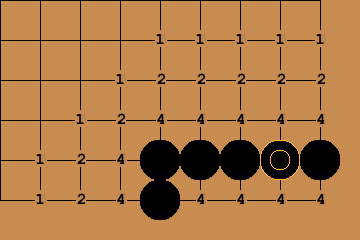
\includegraphics[width=\textwidth]{heur/4a.png}
\caption{Value is halfed each step away from the key group}
\label{fig:heur-4a}
\end{subfigure}
\begin{subfigure}[b]{0.45\textwidth}
\centering
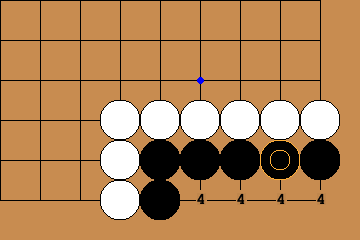
\includegraphics[width=\textwidth]{heur/4b.png}
\caption{White stones devalues moves outside the wall}
\label{fig:heur-4b}
\end{subfigure}
\caption{Distance Based Relevancy}
\label{fig:heur-4}
\end{figure}

The other heuristic method used for move generation is based on pattern matching. Similar to pattern matching for board evaluation, here we use pattern matching to identify relevant moves. The same patterns used for board evaluations are also used to identify relevant moves on the board. The move generator searches for patterns on the board and increments the relevancy score to any moves which are vital points within a pattern found. This will allow the move generator to consider more complex shapes on the board and generate moves according to these shapes. In general, moves found through pattern matching are given higher relevancy score than ones found through the distance-based heuristic. The flaw in this heuristic is of course only a limited number of patterns can be searched because increasing the number of patterns will increase time taken to generate moves hence the same crucial patterns used for board evaluation are used for the move generator.

\begin{figure}[!ht]
\centering
\begin{subfigure}[b]{0.45\textwidth}
\centering
\includegraphics[width=\textwidth]{heur/5a.png}
\caption{Not surrounded by white stones}
\label{fig:heur-5a}
\end{subfigure}
\begin{subfigure}[b]{0.45\textwidth}
\centering
\includegraphics[width=\textwidth]{heur/5b.png}
\caption{Surrounded by white stones}
\label{fig:heur-5b}
\end{subfigure}
\caption{Distance \& Pattern Based Relevancy Combined}
\label{fig:heur-5}
\end{figure}


Relevancy score from the distance-based heuristic and pattern-based heuristic are combined together for each valid move and is ordered into a list from the highest to the lowest relevancy.  Depending on the user’s choice of breadth limit x,  the top x number of moves from this list will be generated and used  within the Alpha-Beta search.~\autoref{fig:heur-5} shows the same board positions shown in  ~\autoref{fig:heur-4} but both the distance-based and pattern-based heuristic applied. We can see that relevancy value for the vital points of the key group is significantly higher than all the other points nearby. The move generator would pick the two vital points as the first two moves to generate which is the best case scenario for the move generator.





\subsection{Suicidal Move Removal}
Keystones are an absolute objective in the program, they are one of the reference points which the program checks to see if the problem is solved or not. From the defender’s perspective, any moves that are detrimental to the immediate safety of keystones need to be removed from the list of valid moves to be searched by the Alpha-Beta algorithm. This entails removing any suicidal moves that decrease the number of liberties of a keystring to 1.

A solution can be derived from the fact that placing 1 stone can at maximum only remove 1 liberty of a keystring. Hence, GoLD only needs to look at the moves that place a stone in liberties of keystrings with 2 liberties, any more liberties would ensure at least 2 liberties would remain intact if a stone was to be placed on a liberty. For a keystring with 2 liberties, placing in one of those 2 liberties does not automatically mean it is a suicidal move for two reasons: Move captures an opponent string; Move would increase or maintain the liberty count. If any of these two reasons are met, then the move is not suicidal.

\begin{itemize}
    \item Both liberties of the keystring is added to the suicidal move list.
    \item Moves that places a stone in the liberty of any opponent string which is in Atari is removed from the suicidal move list.
    \item Moves that connects the keystring to another string which fits the following criteria are removed from the suicidal move list: Must be the same colour as the keystring; Has more than 2 liberties or has 2 liberties which are not the same 2 liberties of the keystring.
    \item Moves that places a stone adjacent to any empty point which is not a liberty of the keystring are removed from the suicidal move list.
\end{itemize}

After these checks are done for all the keystrings, any moves remaining in the suicidal moves list are removed from the valid moves list – this new list of moves is referred to as the good moves list. The good moves list is used during AB search instead of valid moves list to save time by not searching valid moves which would lead to immediate capture of keystones. If no moves are considered “good” then the defending player is to pass instead of making a bad move during AB search.








\chapter{Implementation}
This chapter will go into detail about how GoLD is implemented. GoLD is entirely written in Java and uses a simple 2D game engine called Slick2D [14] which is based on LWJGL [15]. All of the major constructs of Go are implemented within GoLD to create a stable environment for the user to solve life and death problems. Some of the key aspects of the program are the Go board, the Pattern Matcher and the two modes of play. These features were implemented in order to facilitate GoLD's requirements such as the "computer" which plays against the player. Which is essentially a search function greatly dependant on how the Go Board is structured. Many smaller but crucial features had to be implemented to create a completely standalone program which can create and solve problems. To enable complex heuristics to be performed in order to evaluate board positions or generate moves which are relevant, a method of creating and identify patterns of stones is required. A pattern matcher which is able to distinguish between middle, side and corner of the board is built into GoLD.

\section{Board}

The Go board is represented as an object class within GoLD which contains all the vital data to represent the current board position. GoLD's board is designed for the purpose of making tree search and board evaluations as quick as possible. This meant storing more information within the Board object was ideal instead of recalculating information every time it was needed during board evaluation or move generation. The Board object also implements public methods which allow the computer and also the users to interact with the board. The rules of Go are implemented via the Board object which automatically checks if a move played by the user or the computer is valid. If it is valid then the board position is updated to represent the result of the move played otherwise if the move is invalid the Board object denies the move and creates an in-game message to let the user know.
\subsection{Stones}
Representation of stones on the board is simple but effective to keep the operation of gathering information about strings and liberties fast. GoLD takes advantage of Java’s enum type to define the different possible states each intersection on the board could be. While it is possible to represent all the points on the board with simply black, white or empty constants, this would lead to extra operations to distinguish between different types of points such as an empty intersection which is within a problem’s boundaries and an empty intersection which is removed from play. Similar operations are required to distinguish between Ko points and Valid points, black stones and key black stones, white stones and key white stones. To avoid this problem GoLD uses 7 different constants to represent all the intersections on the board. The constants used are BLACK, WHITE, VALID, INVALID, KO, BLACKKEYSTONE, WHITEKEYSTONE . The entire board is represented by a 2D array of enum Stone type.

While the use of a 1D array is possible to represent a 2D Go board and is more space efficient than a 2D array, it would require extra operations to define the board within a 2D coordinate system. This would lead to an extra operation each time the board is accessed which would slow down the entire program.

\subsection{Strings}
A string of stones is any number of stones of the same colour which are connected through adjacent stones of the same colour. A key observation of strings is that once a string is formed, the only way to deform it is through capture by placing on all the liberties of the string. Hence the Board object maintains two collections of strings, one for black and one for white, for the use of the capture functionality. Both collections of strings are updated after each move to represent any changes on the board. Each string is represented by a list of 2D coordinates, due to the lack of an inbuilt tuple type with Java, GoLD uses a custom-built Tuple object to represent 2D coordinates.

\subsection{Capture}
To process capturing of opponent stones, the two collections of strings are used to iterate through each string inside the collection of opponent strings and determine whether any opponent strings lack liberties and if there is a string which do not have any liberties then it is captured. After which the same is done for one's own strings to keep the integrity of the board. If an opponent string has zero liberties, then every stone in the string is replaced by a VALID in the 2D array and the string itself is removed from the collection of opponent strings. Same is applied for one’s own strings but if a capture occurs then the move is invalidated under the self-capture rule.
During this process, two additional information is gathered about the board. For every opponent string if the liberty count is one then the string is considered to be in Atari and hence the intersection of liberty is added on to the opponent’s Atari list which consists all of the opponent’s single liberties and the same applies for the current player's strings. The two Atari list, one for each colour, is maintained within the board and is updated during the process of checking for capture.
The other additional information gathered is whether the Ko rule should be in play the next turn. While checking the opponent’s strings for capture, if a string containing one stone is captured then the intersection of that one stone is in consideration for Ko. After checking for capture, a simple test for Ko is performed. If there is an intersection in considerable for Ko, then the stone placed this turn is checked for the following:

\begin{itemize}
    \item Is the stone in Atari?
    \item Is the stone not connected to any stones of the same colour?
    \item Is the liberty of the stone the same intersection as the one in consideration for Ko?
\end{itemize}

If true for all three questions, then a KO is placed at the intersection which was in consideration for Ko and in the next turn the opponent cannot play there.

\subsection{Valid Move Checker}
Valid move checker is a simple function which returns true or false depending on whether placing on the intersection being checked is valid for the current player. This function consists of three core checks. Is the point being checked on the board? This is in the case of a human player trying to place a stone outside the board grid area. Is the value of that intersection in the board’s 2D array VALID? This is multifunctional as it restricts the user and the computer from playing on points of the board which are removed from play during a problem represented by INVALID and also restricts play on the point of KO. The third check is to make sure that if the current player plays on the point it will not lead to self-capture. The check for self-capture is intricate, the following algorithm is used to determine whether a move is considered self-capture hence invalid.

\begin{algorithm}[H]
\caption{Self-Capture Check}\label{Self-Capture Check}
    \DontPrintSemicolon
    \SetKwFunction{FselfCapture}{selfCapture}
    \SetKwProg{Pn}{Procedure}{:}{}
    \Pn{\FselfCapture{$point$}}{
       \uIf{enemyAtariList.contains(point)}{$\KwRet { true}\;$}
        $ adjacents \gets getAdjancentPoints(point)$\;

        \eIf {(selfAtariList.contains(point))}{
        	\ForEach{adjacent in adjacents}{
        		\uIf{(adjacent is currentColour)}{
        			$adjancentString \gets getString(adjacentPoint)$\;
        			\lIf{($getLiberties(adjacentString).size > 1$)} {$\KwRet { false}\;$}
        		}
        		\ElseIf{(adjacent point is empty)}{$\KwRet { false}\;$}
        	}
    	    {$\KwRet { true}\;$}
	    }{
    	    \ForEach {(adjacent in adjacents)}{
    		    \uIf{(adjacent not enemyColour)} {$\KwRet { false}\;$}
    	    }
    	    {$\KwRet { true}\;$}
	    }
    }
\end{algorithm}

The valid move checker plays an integral part during the tree search which the computer uses to determines the move to play. Every time a new board position is visited by the search, the Alpha-Beta algorithm requires the list of all valid moves in order to generate moves using the move generator and then continue the search by trying out moves generated. To create the list of all valid moves, every point on the board is checked by the valid move checker and if a point is valid then it is added on to the list of valid moves. To reduce redundant processing, the valid moves list is maintained within the Board object and is updated after every move.

\section{Pattern Matcher}
The pattern matcher within GoLD is able to identify a pattern at the 16 possible variations which can occur. A pattern can be rotated at 45° on the board to create 8 different rotations of the same pattern and each pattern can have the colours as normal or inverted hence 16 variations. Specific to the Go board some points are regarded differently to other points and hence the pattern matcher should be able to distinguish between these. The pattern matcher within GoLD is able to define and identify patterns which are on the side, corner or the middle of the board. Note that pattern for the middle of the board can be regarded as a pattern that is allowed to occur anywhere on the board as long as the pattern shape occurs as defined by the pattern.

\subsection{Defining Patterns}
GoLD uses a limited number of predefined patterns which are used within its heuristic pattern matching methods. These predefined patterns are written in simple text notations which are all translated into lists of “Point” objects during the initialisation of static variables. A pattern is just a list of Point objects and these Points are the key components the pattern matcher uses to identify patterns on the board. A Point consists of few fields which allows the pattern matcher to relate each Point to another within a pattern. These fields include two integers which are able to relate each Point inside the pattern to the starting point of the search in terms of distance. The other fields include boolean variables to check whether a Point is on the side, is on the corner, is defending colour or whether it is a wildcard (always matches). The text notation which is used to translate string to a list of Points representing a pattern uses each of characters in the string to create a Point object. ~\autoref{fig:pat-1} shows a Bent Four Corner pattern represented by text notation and the visual representation of the pattern within GoLD. Note here the green stone marked with C shows that the pattern requires that point to be a corner point.


\begin{figure}[!ht]
\centering
\begin{subfigure}[b]{0.2\textwidth}
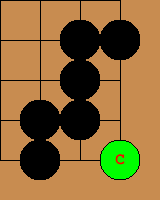
\includegraphics[width=\textwidth]{pat/1.png}
\caption{“xrxldxdxlxdxrr\#”}
\label{fig:pat-1a}
\end{subfigure}
\caption{Visual representation of a pattern}
\label{fig:pat-1}
\end{figure}

\subsection{Matching Patterns}

The patterns matcher itself is based on the idea that every Point object within the pattern is relative x, y distance from the starting point of search. Hence the pattern matcher always deems the starting point as x and y = 0 for the purpose of the pattern matching and then it will search for the rest of the pattern relative to this starting point, starting point is also required to contain a stone. The pattern matcher depends on three parameters, the list of Point object which represents the pattern to look for, a list of intersections all containing stones, as starting points for the pattern matcher and the colour of the defending team. Simple pseudocode for pattern matching algorithm before additional enhancements is shown below.

\begin{algorithm}[H]
\caption{Pattern Matcher}\label{Pattern Matcher}
    \DontPrintSemicolon
    \SetKwFunction{FmatchPattern}{matchPattern}
    \SetKwProg{Pn}{Procedure}{:}{}
    \Pn{\FmatchPattern{$startingPoints,pattern,defColour$}}{
        $matches \gets$ {init list of Tuple lists }\;
        $rotations \gets$ {init list of 8 rotations}\;

        \ForEach{$stuple$ in $startingPoints$}{
            $ matchTries   \gets$ {init list of 8 Tuple lists}\;
            $ skipList  \gets$ {init list of 8 booleans initialised false}\;
            \ForEach{$Point$ in  $pattern$}{
                \lIf{(skipList.allEquals(true))} {$break$}
                 $ checkingTuple \gets$ {$stuple + (Point.x,Point.y)$}\;
                 \ForEach{$rot$ in $rotations$}{
                    \lIf{(skipList[rot]=true)}{break}
                    $ t \gets$ {$checkingTuple.apply(rot)$}\;
                    \uIf{Point.matches(t,defColour)}{
                        $matchTries$.get(rot).add(t)\;
                    }\Else{
                        $skipList[rot] \gets true$\;
                    }

                 }
            }
            \ForEach{$tupleList$ in $matchTries$}{
                \uIf{(TupleList.size() = pattern.size() \textbf{and} !matches.contain(TupleList))}{
                    matches.add(TupleList)
                }

            }

        {$\KwRet { }matches\;$}
        }

    }
\end{algorithm}

The pattern matcher not only returns the matched patterns but also the rotation in which the pattern was found in. GoLD uses the matched patterns along with its rotations to find vital points within each pattern found. Then checks if these vital points are empty, contains defending colour stones or attacking stones to evaluate the value of the overall pattern found. After which more complex checks are performed to see if the pattern identified is fully formed or incomplete, whether the walls of patterns are safe. ~\autoref{fig:pat-2} shows Pyramid Four pattern incomplete where the vital point is not as important, next to a fully complete variation of the same shape where the vital point at a is the only point that matters.

\begin{figure}[!ht]
\centering
\begin{subfigure}[b]{0.45\textwidth}
\centering
\includegraphics[width=\textwidth]{pat/2a.png}
\caption{Incomplete \& unsafe walls}
\label{fig:pat-2a}
\end{subfigure}
\begin{subfigure}[b]{0.45\textwidth}
\centering
\includegraphics[width=\textwidth]{pat/2b.png}
\caption{Complete \& safe walls}
\label{fig:pat-2b}
\end{subfigure}
\caption{Pyramid Four pattern with and without corner stones}
\label{fig:pat-2}
\end{figure}

\section{Modes}

\subsection{Key Features}


\subsection{Differences}




\chapter{Evaluation}


\section{Unit Testing}

\section{Evaluation of Heuristics}
\subsection{Types of Problems}
\subsection{Success Rate}

\section{Beta Testing}
\subsection{Questionnaires}






\chapter{Conclusion}

\section{Summary}

\section{Future Works}

\section{Reflection}


\chapter{References}

1.http://www.cs.cmu.edu/~wjh/go/rules/Japanese.html

2.Müller, M. (2002). POSITION EVALUATION IN COMPUTER GO. ICGA Journal, 25(4), pp.219-228.

3.Chikun, C. (1993). All About Life \& Death. Ishi Pr.

4.Davies, J. (1996). Life and Death. Ishi Pr.

5.Cornelis Diederik van der Werf, E. (2004). AI techniques for the game of Go. [Maastricht]: UPM, Universitaire Pers Maastricht.

6.Akl, S.G., \& Newborn, M. (1977). The principal continuation and the killer heuristic. ACM Annual Conference.

7.Huberman, B.J. (1968). A PROGRAM TO PLAY CHESS END GAMES.

8.Korf R. Depth-first iterative-deepening. Artif Intell. 1985;27(1):97-109. doi:10.1016/0004-3702(85)90084-0

9.https://deepmind.com/research/alphago/

10. Life in the Game of Go  - DAVID B. BENSON*

11.https://webdocs.cs.ualberta.ca/~mmueller/ps/gpw97.pdf  - recognise secure territories

12.https://webdocs.cs.ualberta.ca/~games/go/seminar/2002/020703/ld.pdf -  Static analysis of life and death in the game of Go Ken Chen

13.https://dspace.mit.edu/bitstream/handle/1721.1/50434/41567232-MIT.pdf?sequence=2 -
 A Tsume-Go Life \& Death Problem Solver Adrian B. Danieli

 14. http://slick.ninjacave.com/ - Slick2D

 15. https://www.lwjgl.org/ - LWJGL



 % \begin{figure}[!ht]
 % \centering
 % \begin{subfigure}[b]{0.3\textwidth}
 % \centering
 % 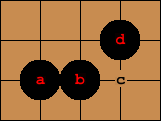
\includegraphics[width=\textwidth]{ex/Ex6-0.png}
 % \caption{Before Move}
 % \label{fig:ex6-0}
 % \end{subfigure}
 % \begin{subfigure}[b]{0.3\textwidth}
 % \centering
 % 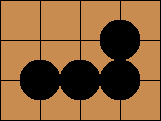
\includegraphics[width=\textwidth]{ex/Ex6-1.png}
 % \caption{After Move}
 % \label{fig:ex6-1}
 % \end{subfigure}
 % \caption{Example 6: The black stones a and b are connected but d is not connected to either a or b. If a black stone is placed at c then a,b,c and d are all said to be connected to each other.}
 % \label{fig:ex6}
 % \end{figure}





\end{document}
